\documentclass[aspectratio=169,11pt]{beamer}

% ---------------------------------------------------------------------------
% Results of Models A, B and C.
% Compile from this folder: pdflatex Presentation.tex (twice).
% Figures come straight from the models' plot folders (\plotsA, \plotsB,
% \plotsC), so rerunning an analysis script updates the slides. Numbers on
% the slides should be copied from the reports, which are reproducible from
% the scripts; every \todo box says which report section to take them from.
% ---------------------------------------------------------------------------

\usepackage{amsmath}
\usepackage{amssymb}
\usepackage{booktabs}
\usepackage{graphicx}
\usepackage{tikz}
\usetikzlibrary{decorations.pathmorphing,positioning,fit,arrows.meta,calc}

% ---- style: Beamer's default theme, colors from the plots' palette --------
\usetheme{default}
\definecolor{plotblue}{HTML}{2A78D6}
\definecolor{plotorange}{HTML}{EB6834}
\definecolor{plotred}{HTML}{E34948}
\definecolor{ink}{HTML}{0B0B0B}
\definecolor{muted}{HTML}{52514E}
\setbeamercolor{frametitle}{fg=plotblue}
\setbeamercolor{title}{fg=plotblue}
\setbeamercolor{structure}{fg=plotblue}
\setbeamercolor{normal text}{fg=ink}
\setbeamercolor{section in toc}{fg=ink}
\setbeamerfont{frametitle}{series=\bfseries}
\setbeamertemplate{navigation symbols}{}
\setbeamertemplate{itemize items}[circle]
\setbeamertemplate{footline}{%
  \hfill{\color{muted}\scriptsize\insertsection\quad\insertframenumber/\inserttotalframenumber}\hspace{1em}\vspace{0.6em}}

% ---- figure folders ----------------------------------------------------------
\newcommand{\plotsA}{../Model_A/Plots_A}
\newcommand{\plotsB}{../Model_B/Plots_B}
\newcommand{\plotsC}{../Model_C/Plots_C}

% ---- helpers -----------------------------------------------------------------
\newcommand{\invlogit}{\operatorname{logit}^{-1}}
\newcommand{\code}[1]{\texttt{#1}}
% visible placeholder for text or numbers still to write; delete when filled
\newcommand{\todo}[1]{{\setlength{\fboxsep}{2pt}\colorbox{plotred!15}{\color{plotred}\scriptsize\textbf{TODO:} #1}}}
% a frame with one figure filling it, plus an optional one-line takeaway
\newcommand{\figframe}[3]{%
  \begin{frame}{#1}
    \centering
    \includegraphics[width=\textwidth,height=0.72\textheight,keepaspectratio]{#2}
    \par\vspace{0.4em}{\small #3}
  \end{frame}}

% ---- trial schematic (slide "The task: one trial") -------------------------
\tikzset{
  handline/.style={line width=1.1pt, line join=round, draw=muted},
  stimprobe/.style={line width=1.3pt, draw=plotblue, decorate,
    decoration={zigzag, amplitude=2.6mm, segment length=3.2mm,
                pre length=5.5mm, post length=5.5mm}},
  distprobe/.style={line width=1.3pt, draw=plotorange, decorate,
    decoration={zigzag, amplitude=1mm, segment length=1.1mm,
                pre length=5mm, post length=5mm}},
  noprobe/.style={line width=1.3pt, draw=plotorange},
  handstroke/.style={handline, fill=white},
  handfill/.style={fill=white},
}
% an open hand, fingers up, at (#1); #2 = 1 (thumb left) or -1 (thumb right); #3 = palm label
\newcommand{\trialhand}[3]{%
  \begin{scope}[shift={(#1)}, scale=1.35]
    \begin{scope}[xscale=#2]
      \clip (-1.5,-0.62) rectangle (1.5,2);
      % outline of the union: stroke every part, then fill every part on top
      \foreach \opt in {handstroke, handfill} {
        \foreach \x/\h in {-0.3/1.25, -0.1/1.42, 0.1/1.36, 0.3/1.15}
          \path[\opt, rounded corners=2.6pt] (\x-0.085,0.4) rectangle (\x+0.085,\h);
        \path[\opt, rotate around={38:(-0.33,0.1)}, rounded corners=2.6pt]
          (-0.42,0.05) rectangle (-0.24,0.78);
        \path[\opt, rounded corners=5pt] (-0.4,-0.05) rectangle (0.4,0.62);
        \path[\opt] (-0.3,-0.8) rectangle (0.3,0.1);
      }
    \end{scope}
    \node[font=\scriptsize, muted] at (0,0.22) {#3};
  \end{scope}}
% one trial panel at x-offset #1; #2 = 1 for bimanual (distractor on), 0 for unimanual
\newcommand{\trialpanel}[2]{%
  \begin{scope}[shift={(#1,0)}]
    \trialhand{0,0}{1}{stim}
    \trialhand{2.6,0}{-1}{dist}
    \draw[stimprobe] (0,2.1) -- (0,4.6);
    \node[plotblue, left] at (-0.35,3.35) {$x_\text{stim}$};
    \ifnum#2=1
      \draw[distprobe] (2.6,2.1) -- (2.6,4.6);
      \node[plotorange, right] at (2.85,3.35) {$x_\text{d}$};
      \node[align=center, font=\small\bfseries] at (1.3,5.35)
        {bimanual trial\\[-1pt]{\normalfont\scriptsize\color{muted}(with distractor)}};
    \else
      \draw[noprobe] (2.6,2.1) -- (2.6,4.6);
      \node[plotorange, right] at (2.7,3.35) {$x_\text{d} = 0$};
      \node[align=center, font=\small\bfseries] at (1.3,5.35)
        {unimanual trial\\[-1pt]{\normalfont\scriptsize\color{muted}(no distractor)}};
    \fi
  \end{scope}}

% ---- graphical models -------------------------------------------------------
\tikzset{
  gm/.style={node distance=1.0cm and 0.8cm},
  latent/.style={circle, draw, minimum size=10mm, inner sep=0pt, font=\small},
  obs/.style={latent, fill=gray!25},
  det/.style={rectangle, draw, minimum size=8mm, inner sep=2pt, font=\small},
  const/.style={font=\small},
  arr/.style={-{Stealth[length=2mm]}},
  plate/.style={draw, rounded corners, inner sep=7pt},
}

% ---- title ---------------------------------------------------------------------
\title{Modeling Bimanual Perceptual Interactions in Macaque Monkeys}
\subtitle{Bayesian Hierarchical Modeling}
\author{Vera Schroeder}
\date{October 29, 2026}

\begin{document}

\begin{frame}
  \titlepage
\end{frame}

\begin{frame}{Outline}
  \tableofcontents
\end{frame}

% ---------------------------------------------------------------------------
% Introduction: task, data, question, modeling approach
% ---------------------------------------------------------------------------
\section{Task and Data}

\begin{frame}{The task}
  \begin{itemize}
    \item The monkey feels a vibration on one finger and reports whether it is
          ``high'' or ``low'' relative to a trained boundary of 28~$\mu m$.
    \item Unimanual trials: stimulus only. Bimanual trials: a distractor vibration on
          the other hand at the same time.
    \item Question: how does the distractor change the categorization?
  \end{itemize}
  \vfill
  \todo{schematic of a trial (stimulus hand, distractor hand, response)}
\end{frame}

\begin{frame}{The data}
  \begin{itemize}
    \item One monkey (Sirius), 42 sessions, 12{,}937 trials.
    \item 8 stimulus amplitudes, 6--50~$\mu m$; 4 groups: hand $\times$
          (unimanual, bimanual).
    \item Each session uses a single distractor amplitude (6--32~$\mu m$) on its
          bimanual trials.
  \end{itemize}
  \vfill
  \todo{figure: raw proportions of ``high'' by amplitude and group}
\end{frame}

\begin{frame}{Psychometric function}
  Every model describes $P(\text{``high''})$ at stimulus $x$ (standardized
  amplitude) by
  \[
    \psi(x) = \gamma_h + (1 - \gamma_h - \gamma_l)\,\invlogit(\beta_0 + \beta_1 x)
  \]
  \begin{itemize}
    \item $\gamma_h$, $\gamma_l$: lapse rates (``high'' to the weakest, ``low'' to the
          strongest stimuli)
    \item Summaries: PSE (where $\psi = 0.5$) and JND (half the distance between
          $\psi = 0.25$ and $0.75$), in $\mu m$
  \end{itemize}
  \vfill
  \todo{one example curve with PSE and JND marked}
\end{frame}

\begin{frame}{Three models}
  \centering
  \begin{tabular}{lll}
    \toprule
    Model & Sessions & Distractor \\
    \midrule
    A & pooled: one curve per group & uni and bi fit separately \\
    B & hierarchical: one curve per group and session & uni and bi fit separately \\
    C & hierarchical, one group per hand & covariate: shift $\beta_2 d$ \\
    \bottomrule
  \end{tabular}
  \vfill
  \raggedright
  For each model: convergence study on synthetic data, then the fit to the real data.
\end{frame}

% !TEX root = ../Presentation.tex
% ---------------------------------------------------------------------------
% Model A: pooled over sessions
% Reports: Model_A/Convergence_A_Report.tex, Model_A/Fit_A_Report.tex
% ---------------------------------------------------------------------------
\section{Model A: Sessions Pooled}

\subsection{Model Structure}

% graphical model, likelihood and priors follow Model_A/Build_Model_A.py and
% Convergence_A_Report, "Model Structure"
\begin{frame}{Model A: graphical model}
  \begin{columns}[c]
    \begin{column}{0.64\textwidth}
      \centering
      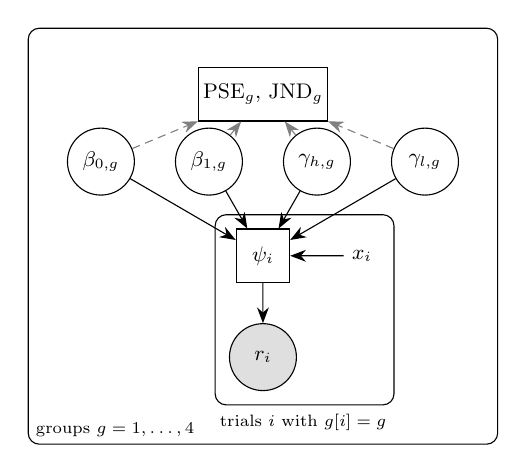
\begin{tikzpicture}[gm, node distance=0.7cm and 0.6cm, scale=0.85, transform shape]
        \node[latent] (b0) {$\beta_{0,g}$};
        \node[latent, right=of b0] (b1) {$\beta_{1,g}$};
        \node[latent, right=of b1] (gh) {$\gamma_{h,g}$};
        \node[latent, right=of gh] (gl) {$\gamma_{l,g}$};
        \node[det, above=0.6cm of $(b1)!0.5!(gh)$] (pse) {PSE$_g$, JND$_g$};

        \node[det, below=1.0cm of $(b1)!0.5!(gh)$] (psi) {$\psi_i$};
        \node[obs, below=0.6cm of psi] (r) {$r_i$};
        \node[const, right=0.8cm of psi] (x) {$x_i$};

        \foreach \p in {b0, b1, gh, gl}
          \draw[arr] (\p) -- (psi);
        \foreach \p in {b0, b1, gh, gl}
          \draw[arr, densely dashed, gray] (\p) -- (pse);
        \draw[arr] (x) -- (psi);
        \draw[arr] (psi) -- (r);

        \node[plate, fit=(x)(psi)(r), inner sep=5pt] (ptrial) {};
        \node[font=\scriptsize, anchor=north east] at (ptrial.south east) {trials $i$ with $g[i]=g$};
        \node[plate, fit=(pse)(b0)(gl)(ptrial), inner sep=14pt] (pgroup) {};
        \node[font=\scriptsize, anchor=south west] at (pgroup.south west) {groups $g = 1,\dots,4$};
      \end{tikzpicture}
    \end{column}
    \begin{column}{0.34\textwidth}
      \footnotesize
      \begin{itemize}
        \item circles: random variables
        \item shaded: observed
        \item rectangles: deterministic
        \item $x_i$: fixed covariate
        \item dashed: derived quantities, not part of the likelihood
      \end{itemize}
    \end{column}
  \end{columns}
\end{frame}

\begin{frame}{Model A: likelihood}
  For trial $i$ in group $g[i] \in \{\text{left\_uni},\ \text{left\_bi},\
  \text{right\_uni},\ \text{right\_bi}\}$:
  \[
    r_i \sim \text{Bernoulli}(\psi_i), \qquad
    \psi_i = \gamma_{h,g[i]} + (1 - \gamma_{h,g[i]} - \gamma_{l,g[i]})\,
             \invlogit(\beta_{0,g[i]} + \beta_{1,g[i]}\, x_i)
  \]
  \begin{itemize}
    \item $r_i = 1$ for ``high'', $0$ for ``low''
    \item $x_i$: stimulus amplitude, standardized by the mean and sd of the 8 levels
    \item One psychometric curve per group, shared by all 42 sessions:
          $4 \times 4 = 16$ parameters
    \item $\psi_i$ clipped to $[10^{-8},\, 1-10^{-8}]$ for numerical stability
  \end{itemize}
  \vfill
  \todo{one-line motivation: simplest model, a baseline}
\end{frame}

\begin{frame}{Model A: priors}
  The same independent priors in every group $g$:
  \begin{align*}
    \beta_{0,g} &\sim \mathcal{N}(0,\ 6) \\
    \beta_{1,g} &\sim \mathcal{N}(4,\ 2) \\
    \gamma_{h,g} &= 0.25\, w_{h,g}, \qquad w_{h,g} \sim \text{Beta}(1.22,\ 4.89) \\
    \gamma_{l,g} &= 0.25\, w_{l,g}, \qquad w_{l,g} \sim \text{Beta}(1.22,\ 4.89)
  \end{align*}
  \begin{itemize}
    \item Beta with mean 0.2, sd 0.15; scaling by 0.25 keeps each lapse rate in
          $(0, 0.25)$, so $\psi$ is increasing and the PSE and JND exist
    \item Implied lapse rate: mean 0.05, 95\% range $[0.003,\ 0.141]$
    \item Not checked by prior predictive simulation
  \end{itemize}
\end{frame}

\figframe{Model A: convergence on synthetic data}
  {\plotsA/Convergence_Plots_A/coverage_vs_size_all_params.png}
  {\todo{takeaway; numbers from Convergence\_A\_Report, ``Conclusions''}}

\figframe{Model A: fit to the real data}
  {\plotsA/Fit_Plots_A/ppc_pooled_by_stimulus.png}
  {\todo{pooled check passes: all 32 proportions inside (Fit\_A\_Report, ``Model Checks'')}}

\figframe{Model A: effect of the distractor}
  {\plotsA/Fit_Plots_A/effect_densities.png}
  {\todo{PSE shift, $\gamma_h$ and JND effects (Fit\_A\_Report, Summary)}}

\figframe{Model A misses the variation between sessions}
  {\plotsA/Fit_Plots_A/ppc_session_cells.png}
  {\todo{within single sessions responses vary more than A predicts (Fit\_A\_Report, ``Model Checks'')}}

% ---------------------------------------------------------------------------
% Model B: hierarchical over sessions; comparison with Model A
% Reports: Model_B/Convergence_B_Report.tex, Model_B/Fit_B_Report.tex,
%          Model_B/Model_Recov_BA_Report.tex
% ---------------------------------------------------------------------------
\section{Model B: Sessions Hierarchical}

\begin{frame}{Model B}
  \begin{itemize}
    \item A curve for every group \emph{and session}, drawn from group-level
          distributions (means and between-session sds).
    \item Design-based priors, checked by prior predictive simulation.
  \end{itemize}
  \vfill
  \todo{plate diagram or equations (Convergence\_B\_Report, ``Model Structure'')}
\end{frame}

\figframe{Model B: convergence on synthetic data}
  {\plotsB/Convergence_Plots_B/hyper_means_recovery_vs_sessions.png}
  {\todo{what is recovered at the real data size (Convergence\_B\_Report, ``Conclusions'')}}

\figframe{Model B: per-session recovery}
  {\plotsB/Convergence_Plots_B/session_params_error_width_coverage_vs_trials.png}
  {\todo{per-session PSE and JND reliable at $\sim$300 trials}}

\figframe{Model B: fit to the real data}
  {\plotsB/Fit_Plots_B/ppc_pooled_by_stimulus.png}
  {\todo{all 32 proportions inside; 99.8\% of session cells (Fit\_B\_Report, ``Posterior predictive checks'')}}

\figframe{Model B: PSE shift in every session}
  {\plotsB/Fit_Plots_B/effect_PSE_by_session.png}
  {\todo{shift negative in 40/42 (left) and 42/42 (right) sessions (Fit\_B\_Report, Summary)}}

\figframe{Model B: the shift grows with distractor amplitude (exploratory)}
  {\plotsB/Fit_Plots_B/effect_vs_distractor_amplitude.png}
  {\todo{about $-2~\mu m$ per 10~$\mu m$; confounded with session order}}

\figframe{Model B against Model A}
  {\plotsB/Fit_Plots_B/effect_A_vs_B.png}
  {\todo{same effects; B better by LOO, 164 (SE 19) (Fit\_B\_Report, ``Comparison with Model A'')}}

\figframe{Is B's advantage real? Model recovery}
  {\plotsB/Model_Recov_Plots_BA/elpd_diff_by_replicate.png}
  {\todo{B wins on all data from B, ties or loses on data from A (Model\_Recov\_BA\_Report)}}

% ---------------------------------------------------------------------------
% Model C: distractor amplitude as a covariate; comparison with Model B
% Reports: Model_C/Convergence_C_Report.tex, Model_C/Fit_C_Report.tex
% ---------------------------------------------------------------------------
\section{Model C: Distractor Amplitude as a Covariate}

\begin{frame}{Model C}
  \[
    \psi(x, d) = \gamma_h + (1 - \gamma_h - \gamma_l)\,
                 \invlogit(\beta_0 + \beta_1 x + \beta_2 d)
  \]
  \begin{itemize}
    \item $d$: distractor amplitude (0 on unimanual trials); one group per hand.
    \item Uni- and bimanual trials share slope and lapse rates: the distractor only
          shifts the curve, by an amount proportional to $d$.
  \end{itemize}
  \vfill
  \todo{why: test the amplitude trend from Model B inside a model}
\end{frame}

\figframe{Model C: prior on the distractor effect}
  {\plotsC/Convergence_Plots_C/Prior_Check_C_distractor.png}
  {\todo{weakly informative; a weak distractor can only shift a little (Convergence\_C\_Report)}}

\figframe{Model C: convergence on synthetic data}
  {\plotsC/Convergence_Plots_C/hyper_means_recovery_vs_sessions.png}
  {\todo{all hand-level means recovered, $\mu_{\beta_2}$ well (Convergence\_C\_Report, ``Conclusions'')}}

\figframe{Model C: per-session $\beta_2$ is weak for small distractors}
  {\plotsC/Convergence_Plots_C/session_b2_true_vs_recovered.png}
  {\todo{shrinkage toward the hand mean at 6~$\mu m$}}

\figframe{Model C: the shift grows with distractor amplitude}
  {\plotsC/Fit_Plots_C/pse_shift_vs_amplitude.png}
  {\todo{$\mu_{\beta_2}$ and the typical shift at 6 and 32~$\mu m$ (Fit\_C\_Report, ``Effect of the Distractor'')}}

\figframe{Model C misfits at the weakest stimuli}
  {\plotsC/Fit_Plots_C/ppc_pooled_by_stimulus.png}
  {\todo{shared lapse rates: 6 of 32 proportions outside (Fit\_C\_Report, ``Posterior predictive check'')}}

\figframe{Model C against Model B}
  {\plotsC/Fit_Plots_C/pse_shift_C_vs_B.png}
  {\todo{LOO favors B by 37 (SE 12); 6~$\mu m$ shifts too small (Fit\_C\_Report, Comparison)}}

\figframe{Model C: shift by distractor amplitude, observed vs predicted}
  {\plotsC/Fit_Plots_C/ppc_by_distractor_amplitude.png}
  {\todo{right hand at 6~$\mu m$ outside: a presence effect (Fit\_C\_Report, amplitude check)}}

% !TEX root = ../Presentation.tex
% ---------------------------------------------------------------------------
% Summary and next steps
% ---------------------------------------------------------------------------
\section{Summary}

\begin{frame}{Comparison of the models}
  \centering
  \begin{tabular}{lccc}
    \toprule
     & A & B & C \\
    \midrule
    Sessions & pooled & hierarchical & hierarchical \\
    Distractor & separate groups & separate groups & covariate $\beta_2 d$ \\
    $\text{elpd}_\text{loo}$ & \todo{} & \todo{} & \todo{} \\
    PSE shift, left / right ($\mu m$) & \todo{} & \todo{} & \todo{} \\
    \bottomrule
  \end{tabular}
  \vfill
  \raggedright
  \todo{fill from Fit\_A/B/C\_Report; elpd differences from Fit\_B and Fit\_C}
\end{frame}

\begin{frame}{Conclusions}
  \begin{itemize}
    \item The distractor lowers the PSE: \todo{size, both hands}.
    \item It raises the rate of ``high'' responses to weak stimuli ($\gamma_h$).
    \item The sessions differ; a hierarchical model is needed.
    \item The shift grows with distractor amplitude, \todo{but not proportionally?}
  \end{itemize}
\end{frame}

\begin{frame}{Next steps}
  \begin{itemize}
    \item Revise Model C: lapse rates per condition, a distractor-presence term,
          possibly a bimanual slope.
    \item Model recovery for B against the revised C.
    \item \todo{further data or experiments}
  \end{itemize}
\end{frame}


\appendix
%%% !TEX root = ../Presentation.tex
% ---------------------------------------------------------------------------
% Backup slides (after \appendix): diagnostics and details for questions
% ---------------------------------------------------------------------------
\section{Backup}

\figframe{Backup: Model B sampling diagnostics}
  {\plotsB/Fit_Plots_B/trace_session_params_left_bi.png}
  {\todo{no divergences, $\hat{R} = 1.00$ (Fit\_B\_Report, ``Sampling diagnostics'')}}

\figframe{Backup: Model C sampling diagnostics}
  {\plotsC/Fit_Plots_C/trace_session_params_left.png}
  {\todo{2 divergences in 20{,}000 draws, $\hat{R} = 1.000$ (Fit\_C\_Report)}}

\figframe{Backup: Model C session PSEs}
  {\plotsC/Fit_Plots_C/PSE_by_session.png}
  {}


\end{document}
